\section{Fast precision estimation in high‐dimensional multivariate joint models}


\subsection{Introduction}
\label{sec_intro}

There are different approaches to deal with modelling multivariate clustered data. Authors like \cite{pawitan1993} proposed to analyze each response conditioned on all the others. As an alternative, one may specify a marginal model for each response separately and then join them using an appropriate way. Among such ways are using a latent variable \citep{catalano1992}, copulas \citep{nelsen2007}, or random effects \citep{laird1982}. The latter is of interest in this short note. 

%In the joint modelling approach of multivariate repeated measurements data using random effects, a mixed model is considered for each response separately. Then, the random effects of these models are considered to follow a multivariate distribution which would reflect the association between different responses.

Let $y_{rij}$ be the $j$th measurement taken on the $i$th cluster for the $r$th outcome, $i=1,\ldots,N$, $r=1,\ldots,m$ and $j=1,\ldots,n_{ri}$. Obviously, the number of measurements available for subject $i$ is $\sum_{r=1}^m n_{ri}$. Note that the various outcomes do not need to be of the same kind (continuous, binary, count data, etc.). Also there is no need to have sequences of the same length for each cluster or each outcome. Let $\mathbf{Y_{ri}}$ be the $n_{ri}$ measurements taken on cluster $i$ for outcome $r$. The model assumes that each $\mathbf{Y_{ij}}$ satisfies a mixed model:
\begin{equation}
\label{mixed_model}
\mathbf{Y_{ri}} = \boldsymbol{\mu_{ri}} + \epsilon_{ri},
\end{equation}
where
\begin{equation}
\label{mu_function}
\mathbf{\mu_{ri}} = \mathbf{h}(X_{ri} \boldsymbol{\beta_r} + Z_{ri} \mathbf{b_{ri}}).
\end{equation}
As one may see in (\ref{mu_function}), each outcome can have its own set of fixed effects. In order to capture the associations between different responses, the mixed model approach for joint modelling of the $m$ outcomes allows for correlation between the random effects of each outcome. Let $\mathbf{b_i} = (\mathbf{b_{1i}},\ldots,\mathbf{b_{mi}})'$; the joint model assumes:
\begin{equation}
\label{random_effect_dist}
\mathbf{b_i}=
\begin{bmatrix}
b_{1i} \\
b_{2i}\\
\vdots\\
b_{mi}\\
\end{bmatrix} \sim N \left ( 
\begin{bmatrix}
0 \\
0\\
\vdots\\
0\\
\end{bmatrix}, 
D=\begin{bmatrix}
D_{11} & D_{12} & \ldots & D_{1m}\\
D_{21} & D_{22} & \ldots & D_{2r}\\
\vdots & \vdots & \ddots & \vdots\\
D_{m1} & D_{r2} & \ldots & D_{mm}\\
\end{bmatrix}
\right).
\end{equation}
The matrix $D_{rs}$ ($r,s=1,\ldots,m$) represents the covariance between $\mathbf{b_{ri}}$ and $\mathbf{b_{si}}$. 

While using the joint modelling approach for the multivariate clustered data is a flexible methodology, it can easily become intractable when the number of outcomes becomes large. As the matrix D contains the association between all outcome sequences, its dimension can quickly grow large. Therefore, it is easily possible that such a flexible joint model cannot be used in practice. 

In order to overcome this drawback, \cite{Verbeke2006} and \cite{Verbeke2007} proposed a pseudo-likelihood based approach which considers all possible pairs (or higher order subsets) of the $r$ outcomes and fit them separately. Obviously, using this methodology some parameters are estimated more than once. Averaging multiply estimated parameters gives a final estimate for each parameter. To find a correct estimate of the variance, \cite{Verbeke2006} and \cite{Verbeke2007} proposed a sandwich-type correction of the form $J^{-1}KJ^{-1}$, where $J$ and $K$ are formed based on cluster-wise Hessians and gradients of the log-pseudo-likelihood function, respectively. 

The need for cluster-wise derivatives of the first and second order makes computing this sandwich estimator difficult and possibly expensive. \cite{pair_lin} and \cite{kundu} provided {\tt{SAS}} implementations for the case of linear mixed models. Also, \cite{pair_gen} considered the case of generalized linear models using {\tt{Proc NLMIXED}} in {\tt{SAS}}. However, the cluster-wise calculation can become very expensive for large samples. Also, the focus of these implementations is on the fixed effects only. Implementing the variance estimation for, e.g., matrix $D$ (\ref{random_effect_dist}) is far more complicated. Also, obtaining the right precision quantities in commonly available software like {\tt{R}} demands new implementations. Furthermore, a different model needs its own implementation which includes evaluating gradients and Hessians of the log-(pseudo-)likelihood function. 

\cite{hoffman2001} proposed within-cluster re-sampling to analyze clustered data when the intra-class correlation is considered a nuisance. Their idea was explored in \cite{follmann2003} who gave it the name multiple outputation (MO). MO consists of repeatedly taking sub-samples of size $1$ from each cluster to form a sub-sample of independent observations, to then apply the standard methodologies for such data. The estimated parameters  and their precisions from several sub-samples will be combined using appropriate rules. \cite{hoffman2001} have shown that their variance estimator is consistent.



{\color{black}{Note that using pairs of variables instead of analyzing them jointly is a trick which is not restricted to likelihood-based methods. It has been used in different contexts. For example, \cite{aas2009} have used pair-copulas to model complex multivariate dependencies. Especially with Gaussian outcomes, pairwise approaches (e.g., vine copulas) allow retrieval of the full multivariate association structure, without the need for full joint modelling.}}



In this short note we extend the idea of MO to compute the variance of a pairwise-fitted multivariate joint model as a faster and easier way. The MO-based correction for the variance will be presented in Section~\ref{sec_method}. A simulation study will compare its performance with a sandwich correction in Section~\ref{sec_sim}. The two corrections are compared in analyzing a real dataset in Section~\ref{sec_application}, and finally the paper is concluded in Section~\ref{sec_conclusions}.

\subsection{A fast variance estimator based on multiple outputation}
\label{sec_method}
Consider $y^{(s)}_{rij}$ as the $j$th measurement on $i$th cluster for $r$th outcome in the $s$th sub-sample, where $s=1,\ldots ,M$, $j=1,\ldots,n_{ri}$, $i\in \{1,\ldots,N\}$, and $r\in \{1,\ldots,m\}$. Also consider $\boldsymbol{\theta}^{(s)}$ a vector of size $p_s$ ($s=1,\ldots,M$), containing parameters estimated using the variables involved in the $s$th sub-sample, obviously, $\boldsymbol{\theta}^{(s)} \subseteq \boldsymbol{\theta}$. Let $\boldsymbol{\Theta}' = (\boldsymbol{\theta}^{(1)},\ldots,\boldsymbol{\theta}^{(M)})$ the stacked vector combining all parameters estimated in different sub-samples. $\widehat{\boldsymbol{\Theta}}$ replaces each $\boldsymbol{\theta}^{(s)}$ by its estimate. Also, $\boldsymbol{\Sigma}_{\boldsymbol{\Theta}}$ is a vector of length $\sum_{s=1}^M\times p_s$, with its elements the variance of each element of $\widehat{\boldsymbol{\Theta}}$.


The MO in the current paper extends the one in \cite{hoffman2001} and \cite{follmann2003} in two main directions. First, the sub-samples in our approach are of size larger than one. The second aspect of our proposed extension of MO concerns the sub-sampling scheme. The MO in the sense of \cite{hoffman2001} and \cite{follmann2003} takes random sub-samples of size $1$ from each cluster many times to form sub-samples of independent observations. In our approach, the sub-samples are not taken at random but based on a pre-defined structure which implies a fixed number of needed sub-samples.  {\color{black}{{One may note that the sub-sampling in our proposal is performed at the response level. Therefore, as it is not necessary to measure every response for all subjects, each subject will be presented in the sub-samples which the responses presented there are measured for it.}}} 

For example, using a pairwise approach, each sub-sample consists of all the observations available for each subject corresponding to the two outcomes in the pair under analysis. Therefore, having $m$ outcomes, we need to take $M=m(m-1)/2$ sub-samples, each with a size larger than one. Note that, in a pairwise approach, $M=m(m-1)/2$ is the number of all possible sub-samples. Taking less sub-samples would fail to estimate some parameters. On other hand, taking more sub-samples is not possible without repeating some already taken sub-samples.  {\color{black}{{As it was remarked, it is not necessary for every subject to be present in every sub-sample. In a pairwise approach, suppose we only have three responses $y_1,y_2,y_3$ and for a particular subject only $y_1$ is measured. Then this subject will only be present in pairs $(y_1,y_2)$ and $(y_1,y_3)$.}}}


%Note that in a pairwise modelling approach, each sub-sample consists of the measurements corresponding to one pair of outcomes. Therefore, having $m$ outcomes, we have $M=m(m-1)/2$ sub-samples. For example, the sub-sample corresponding to the first pair (first and second responses) would consists of $\sum_{j=1}^K (n_{1j}+n_{2j})$ observations. This can be considered an extension of MO in the sense of \cite{hoffman2001} and \cite{follmann2003} that takes sub-samples of size one from each cluster.



As one may have already noticed, some of the parameters in $\boldsymbol{\theta}$ would have more than one counterpart in $\boldsymbol{\Theta}$. In order to bring the $\boldsymbol{\Theta}$ back to the desired parameter space, one may take the average of possible several counterparts of each element of $\boldsymbol{\theta}$ in $\boldsymbol{\Theta}$. This can be done using an appropriate weight matrix pre-multiplied by $\boldsymbol{\Theta}$. Consider $A$, a $(p\times \sum_{s=1}^M p_s)$ matrix where its $(\ell,k)$th element, $\ell=1,\ldots,p$, $k=1,\ldots, (p\times \sum_{s=1}^M p_s)$, is defined as follows:


\begin{equation}
\label{matrix_A}
A_{\ell,k} = \left\{
\begin{array}{rl}
1 & \text{if } \boldsymbol{\Theta}_{k} \text{ is a {\color{black}{component}} of } \boldsymbol{\theta}_{\ell},\\
0 & \text{otherwise},
\end{array} \right.
\end{equation}


where $\boldsymbol{\Theta}_{k}$ and $\boldsymbol{\theta}_{\ell}$ are the $k$th and $\ell$th elements in $\boldsymbol{\Theta}$ and $\boldsymbol{\theta}$, respectively. If $W$ is defined as $A$ but with the rows divided by their sum then the combination rules for combining the estimates from $M$ sub-samples are as follows,
%\begin{equation}
%\label{comb_rules}
%\begin{cases}
%\widetilde{\boldsymbol{\theta}} = W \widehat{\boldsymbol{\Theta}},\\
%\mathrm{diag}\left\{\mathrm{Var}(\widetilde{\boldsymbol{\theta}} )\right\}=  W \boldsymbol{\Sigma}_{\boldsymbol{\Theta}} - \mathrm{diag}\left\{W \left(\widehat{\boldsymbol{\Theta}}-\bar{\boldsymbol{\Theta}} \right) \left(\widehat{\boldsymbol{\Theta}}-\bar{\boldsymbol{\Theta}} \right)' W'\right\},
%\end{cases}
%\end{equation}



\begin{equation}
\label{comb_rules}
\begin{cases}
\widetilde{\boldsymbol{\theta}} = W \widehat{\boldsymbol{\Theta}},\\
{\color{black}{\mathrm{diag}\left\{\mathrm{Var}(\widetilde{\boldsymbol{\theta}} )\right\}=  W \boldsymbol{\Sigma}_{\boldsymbol{\Theta}} - W \mathrm{diag}\left\{\left(\widehat{\boldsymbol{\Theta}}-\bar{\boldsymbol{\Theta}} \right) \left(\widehat{\boldsymbol{\Theta}}-\bar{\boldsymbol{\Theta}} \right)' \right\}}},
\end{cases}
\end{equation}

where $A'$ is the transpose of $A$, and $\bar{\boldsymbol{\Theta}} = \widehat{\boldsymbol{\Theta}} - A' \tilde{\boldsymbol{\theta}}$. For the proof, see \citet[][Appendix 2]{hoffman2001}. These authors have shown that $I^{1/2} ( \widetilde{\boldsymbol{\theta}} - \boldsymbol{\theta}) \xrightarrow{d} N(0, \Sigma)$, where $\xrightarrow{d}$ means convergence in distribution and $\mathrm{Var}(\widetilde{\boldsymbol{\theta}} )$ is a consistent estimator of $\Sigma$.

We may note that the combination rules in (\ref{comb_rules}) are only estimating the diagonal elements of the covariance matrix of $\widetilde{\boldsymbol{\theta}}$.  If one is interested in estimating the off-diagonal elements as well, the combination rules are the same. One would only need to construct $\boldsymbol{\Sigma}_{\boldsymbol{\Theta}}$, which takes into account the off-diagonal elements also, then an appropriate $W$ can be used to combine the estimated variances and covariances obtained from each sub-sample. The corresponding vector of unique parameters in this covariance matrix would be $p(p+1)/2$, where each sub-sample would estimate part of them. 


{\color{black}{As one may see in (\ref{comb_rules}), the combination rule for the variance has a subtraction, so as pointed out by both \cite{hoffman2001} and \cite{follmann2003}, theoretically, it is possible to estimate a non-positive definite covariance matrix. Although the chance for such an occurrence is small, and we have not observed it even once in our simulations, it is still necessary to discuss this matter. We can consider three situations in which such a phenomenon would occur: (1) the sample size, $N$, is not sufficiently large, (2) the number of sub-samples, $M$, is not sufficiently large, and (3) the size of each sub-sample is not sufficiently large.

\cite{hoffman2001} proposed to increase the number of sub-samples, $M$, to solve this problem. As it was pointed out, unlike the usual MO, in our approach the number of sub-samples is fixed. Therefore, in case of a non-positive definite covariance estimate, we suggest to take larger sub-samples each time. Note that taking such a strategy is not possible in the usual MO, since it takes one observation per cluster, so the sub-sampling size is fixed. Taking larger sub-samples in our case means to consider triples, quadruples, etc., instead of pairs. We expect the problem of non-positive definite covariance estimate to vanish when taking larger sub-samples. 

When maximum likelihood estimator (MLE) is used, \cite{follmann2003} proposed a variance estimator based on MLE approximation, using first order Taylor expansion of the score function. This approach requires the evaluation of the subject-wise gradient and Hessian of the log-likelihood function, which is similar to the requirements of the sandwich estimator. Therefore, in case where even with larger sub-samples a non-positive definite covariance estimate persists, we suggest to use the sandwich estimator instead of MO.}} 





\subsection{Simulations}
\label{sec_sim}
In this section the proposed idea will be explored and examined via two simulations studies. Sub-section~\ref{subsec_lin} considers joint modelling of linear mixed models, and Sub-section~\ref{subsec_genlin} takes a joint model of ordinal data in a generalized linear mixed models context.

\subsubsection{Gaussian responses}
\label{subsec_lin}
Consider the linear case with identity link in (\ref{mu_function}), as follows:
\begin{equation}
\label{lin_mixed}
\BY_i= X_i \beta + Z_i \Bb_i + \epsilon_i,
\end{equation}
where $X_i$ is the design matrix regarding fixed effects, $\beta$ represents the fixed effects, $Z_i$ is the design matrix related to the random effects, and $\Bb\sim N(0,D)$ shows the random effects. The errors are represented by $\epsilon_i\sim N(0,R)$. In order to evaluate the proposed method in a simulation study, consider the model in (\ref{lin_mixed}) with parameters:

\begin{equation}
\label{sim_params}
\beta=(5,5,5,5), D= \left(
\begin{array}{cccc}
60 & 40 & 25 & 40 \\
& 50 & 35& 30 \\
& & 45 & 40 \\
&&&55
\end{array} \right), R= 196 I_{n_i},
\end{equation}
where $I_{n_i}$ is the identity matrix of order $n_i$, with $n_i$ the length of the $i$-th cluster. {\color{black}{This means that both of the $X_i$ and $Z_i$ are formed by columns of $1$'s.}} The data are generated from such model 100 times, each consists of 100 clusters of size $n_i=5$. The mixed model is fitted to the full sample as well as each of the 6 pairs using Proc MIXED in {\tt{SAS}}. Then, the estimates and variances are combined using (\ref{comb_rules}). Also, the sandwich estimator is calculated using {\tt{\%jointpair}} macro in {\tt{SAS}} in \cite{pair_lin}.

Figure \ref{fig_sim} shows the simulation results. As one may see, the relative efficiency of estimating fixed effects using sandwich and MO corrections are very similar. Furthermore, the relative efficiency for estimating parameters in the $D$ matrix are also presented. These parameters are only estimated using the MO correction, as the implementation was not available for sandwich-correction. The interesting result here is the computation time. As one may see, using MO-correction the computation can be done more than 2500 times faster. On the other hand, in case that computing the full likelihood model is possible (as it is the case in our simulation study), MO-correction can also possibly be computed faster than the full-likelihood. Therefore, it is not only an alternative for infeasible likelihoods, but also, it can be used to accelerate computations that are strictly speaking doable.

%\begin{figure}
%\centering
%\includegraphics[width=\textwidth,trim=0 110 0 120]{fig_sim.eps}
%\caption{Histogram of computation time using IMO and sandwich corrections.} 
%\label{fig_scatter2}
%\end{figure} 


\begin{figure}[htb]
\begin{center}
\includegraphics[width=\textwidth]{fig_sim_eq_new.eps}
\caption{Simulations {\color{black}{(Gaussian outcomes)}}. Top: Relative efficiency of estimated fixed effects using MO-correction (left) and sandwich-correction (middle), estimated $D$-matrix using MO-correction (right) compared to the full model. {\color{black}{The relative efficiency is defined as the ratio of the variance of the alternative method and the full likelihood, e.g., for MO $\mathrm{Var}(\widetilde{\theta}_{\mathrm{MO}})/\mathrm{Var}(\widehat{\theta}_{\mathrm{full}})$ is computed}}. Bottom: Histograms of computation time (in seconds) using sandwich and MO corrections (first and second). Histograms of computation time (in seconds) using sandwich and MO corrections (third and fourth) relative to the full model computation time.}
\label{fig_sim}
\end{center}
\end{figure}



{\color{black}{
In order to see how our proposal performs comparing with sandwich estimator when the correlation between the random effects is small, the simulation above is repeated, but this time the off-diagonal elements of $D$ matrix in (\ref{sim_params}) are divided by $10$. Figure~\ref{fig_sim_small} shows the relative efficiencies of the variances obtained using MO and sandwich corrections. As one may see, these relative efficiencies are again very close to $1$.

\begin{figure}[htb]
\begin{center}
\includegraphics[width=\textwidth]{fig_sim_small.eps}
\caption{{{Simulations (Gaussian outcomes). Top: Relative efficiency of estimated fixed effects using MO-correction (left) and sandwich-correction (right). Bottom: estimated $D$-matrix using MO-correction compared to the full model. The relative efficiency is defined as the ratio of the variance of the alternative method and the full likelihood, e.g., for MO $\mathrm{Var}(\widetilde{\theta}_{\mathrm{MO}})/\mathrm{Var}(\widehat{\theta}_{\mathrm{full}})$ is computed.}}}
\label{fig_sim_small}
\end{center}
\end{figure}
}}



{\color{black}{

\subsubsection{Non-Gaussian responses}
\label{subsec_genlin}

In order to investigate the performance of our proposal for non-Gaussian responses and more complex models a simulation is done based on the Leuven diabetes project. This dataset is analyzed in \cite{ivanova2015}, details about this study can be found there. Here we only review parts necessary for our simulations. In order to study how well the diabetes is controlled, three outcomes were measured for each patient at baseline ($T_0$) and one year later ($T_1$). These three outcomes of interest were LDL-cholesterol (low-density lipoprotein cholesterol, mg/dl), HbA1c (glycosylated hemoglobin, \%), and SBP (systolic blood pressure, mmHg). Although these three variables are continuous, the interest was in expert-specified cut-off values of these outcomes. The cut-off values are defined as $\{<100, [100,115), [115, 130),\geq 130 \}$ (mg/dl) for LDL-cholesterol, $\{<7, [7, 8), \geq 8\}\%$ for HbA1c, and $\{ \leq 130, (30,140],(140,160],>160\}$mmHg for SBP.

In order to analyze these 3 ordinal outcomes together, a joint modelling approach with a proportional odds mixed model (POMM) for each response was considered in \cite{ivanova2015}. The POMM for each response is as follows:
\begin{equation}
\label{sim2_model}
\mathrm{logit}[P(Y_{rij}<k)] = \xi_{r0k} + \xi_{r1} t_{ij} + \xi_{r2} X_{i} + b_{ri} + \epsilon_{rij},
\end{equation}
where $r=1,2,3$ indicates the outcome of interest, and $k=1,\ldots,K-1$ with $K$ as the number of levels of the corresponding outcome of interest. Furthermore, $X_i$ shows the gender of the subject, and $b_{ri}$'s are the random intercepts corresponding to each outcome. Following the mixed model approach for joint modelling of multiple outcomes, we assume the three random intercepts to be normally distributed with the following covariance matrix.

\begin{equation}
\label{sim2_random_effect_dist}
\begin{bmatrix}
b_{1i} \\
b_{2i}\\
b_{3i}\\
\end{bmatrix} \sim N \left ( 
\begin{bmatrix}
0 \\
0\\
0\\
\end{bmatrix}, 
D=\begin{bmatrix}
D_{11} & D_{12} & D_{13}\\
 & D_{22} & D_{23}\\
&& D_{33}\\
\end{bmatrix}
\right).
\end{equation}
The parameter values for generating the data were obtained by fitting the joint model to the Leuven diabetes dataset. The data were generated $200$ times using {\tt{SAS Proc IML}}. Each time the parameters in the $3$ pairs were estimated using adaptive Gaussian quadrature \citep{pinheiro1995} with $3$ quadrature points in {\tt{SAS Proc NLMIXED}} and the combined variance was estimated using sandwich and MO corrections. Considering the complexity of the model, in order to do the simulation quicker, the codes were run on VSC cluster in Leuven, Belgium.

The results of the simulations are summarized in Table~\ref{tab_sim2}. Column 3 of Table~\ref{tab_sim2} shows the parameter values which were used to generate the data. The last three columns show the means and standard deviations over 200 replications for estimated variance using MO, sandwich, and their relative efficiency, respectively. As one may see, for all of the variables the estimated variances are very close, therefore, one can conclude that our proposal performs well also in a complex model with non-Gaussian responses.

\begin{table}[ht]
\centering
{{
\caption{Simulations (non-Gaussian outcomes). The estimated model for three ordinal outcomes. The first columns indicates different outcomes, and the second columnn shows the estimated effect. The data obtained parameter-values which were used to generate the data are presented in column 3. Columns four and five show the average (standard deviation) of standard error using MO and sandwich, obtained over 200 replications, respectively. The last column shows the relative efficiency of MO compared to sandwich: $\mathrm{Var}(\widetilde{\theta}_{\mathrm{MO}})/\mathrm{Var}(\widetilde{\theta}_{\mathrm{Sandwich}})$.}
\label{tab_sim2}
\resizebox{\textwidth}{!}{\begin{tabular}{lllccc}
  \hline
Outcome&Effect&Parameter & MO & Sandiwch & ARE (MO/Sandwich)  \\ 
  \hline \vspace*{1mm} 
\multirow{4}{*}{LDL-chol.}&Int. 1&$\xi_{101}=-0.740$ & 0.039 (0.006) & 0.039 (0.006) & 0.993 (0.009)  \\ \vspace*{1mm} 
&Int. 2&  $\xi_{102}=0.480$ & 0.038 (0.006) & 0.038 (0.006) & 0.998 (0.009)  \\ \vspace*{1mm} 
&Int. 3 & $\xi_{103}=1.580$ & 0.042 (0.006) & 0.041 (0.007) & 1.012 (0.010)  \\ \vspace*{1mm} 
&Time  &$\xi_{11}=1.050$ & 0.032 (0.004) & 0.032 (0.004) & 1.024 (0.008)  \\ \vspace*{1mm} 
&Gender  &$\xi_{12}=0.450$ & 0.048 (0.008) & 0.048 (0.008) & 0.989 (0.001) \\ \vspace*{1mm} 
&RI sd  &$\sqrt{D_{11}}=1.880$ & 0.036 (0.005) & 0.034 (0.005) & 1.105 (0.010)  \\ \vspace*{1mm} 
\multirow{3}{*}{HbA1c}&Int. 1  &$\xi_{201}=270$ & 0.042 (0.007) & 0.042 (0.007) & 0.997 (0.008)  \\ \vspace*{1mm} 
&Int. 2  &$\xi_{202}=2.610$ & 0.052 (0.009) & 0.051 (0.009) & 1.043 (0.010)  \\ \vspace*{1mm} 
&Time  &$\xi_{21}=1.040$ & 0.036 (0.004) & 0.035 (0.005) & 1.034 (0.010)  \\ \vspace*{1mm} 
&Gender  &$\xi_{22}=-0.090$ & 0.054 (0.009) & 0.054 (0.009) & 0.979 (0.001)  \\ \vspace*{1mm} 
&RI sd  &$\sqrt{D_{22}}=2.150$ & 0.042 (0.007) & 0.040 (0.007) & 1.131 (0.012)  \\ \vspace*{1mm} 
\multirow{4}{*}{SBP}&Int. 1   &$\xi_{301}=-0.190$ & 0.035 (0.006) & 0.035 (0.006) & 0.995 (0.009)  \\ \vspace*{1mm} 
&Int. 2   &$\xi_{302}=1.380$ & 0.038 (0.007) & 0.038 (0.007) & 1.012 (0.009)  \\ \vspace*{1mm} 
&Int. 3   &$\xi_{303}=3.700$ & 0.056 (0.009) & 0.055 (0.010) & 1.028 (0.015)  \\ \vspace*{1mm} 
&Time   &$\xi_{31}=0.510$ & 0.030 (0.003) & 0.030 (0.003) & 1.013 (0.005)  \\ \vspace*{1mm} 
&Gender   &$\xi_{32}=0.190$ & 0.044 (0.008) & 0.044 (0.008) & 0.991 (0.001)  \\ \vspace*{1mm} 
&RI sd  &$\sqrt{D_{22}}=1.620$ & 0.034 (0.004) & 0.033 (0.005) & 1.073 (0.015)  \\ \vspace*{1mm} 
LDL-col. vs. HbA1c&Cov RI's &$D_{12}=0.808$ & 0.067 (0.013) & 0.068 (0.014) & 0.961 (0.014)  \\ \vspace*{1mm} 
LDL-col. vs. SPB&Cov RI's  &$D_{13}=1.218$ & 0.057 (0.012) & 0.057 (0.012) & 0.994 (0.015)  \\ \vspace*{1mm} 
HbA1c vs. SBP&Cov RI's   &$D_{23}=1.393$ & 0.065 (0.014) & 0.065 (0.014) & 0.993 (0.016)  \\ 
   \hline
\end{tabular}} }}
\end{table}

}}


\subsection{Application}
\label{sec_application}
To evaluate the hearing performance of a subject, hearing threshold sound pressure levels (measured in dB) are considered. By definition, a hearing threshold is the lowest signal intensity possible to perceive by a subject at a specific frequency. In a study considered in \cite{Molenberghs2000} and \cite{Verbeke2006}, hearing threshold measured in 11 different frequencies between 125 Hz and 8000 Hz for left and right ears obtained on 603 male participants from the Baltimore Longitudinal Study of Ageing, BLSA \citep{shock1984}. The number of visits for each subject which varies between 1 to 15 are unequally spaced. In this illustration all subjects with missing values are ignored to make a fair comparison between MO and sandwich corrections.

In order to model different frequencies simultaneously, \cite{Verbeke2006} used a joint model approach. Because of several outcomes of interest, they have proposed a pairwise approach to jointly fit the model to the data. In this section we use this dataset to illustrate our proposal and compare it with the sandwich correction proposed in \cite{Verbeke2006}. Consider $y_i(t)$ as the hearing threshold for subject $i$ at time $t$ for some frequency. The mixed model fitted to this single response is as follows:

\begin{equation}
\label{application_model}
y_i(t)=(\beta_1 +\beta_2 Age_i + \beta_3 Age_i^2 + a_i) + (\beta_4 + \beta_5 \mathrm{Age}_i + b_i)t + \beta_6 V(t) + \epsilon_i(t),
\end{equation}
where $t$ represents time and $V(t)$ is a dummy variable indicating whether the measurement is taken at the first time visit to account for systematically higher response values at the first visit. Also, $Age$ indicates the age of the participant at first visit. Furthermore, $a_i$ and $b_i$ are the random intercepts and slopes, respectively; and $\epsilon$ is the error term. Using a joint modelling approach to model the hearing threshold at several frequencies one needs to let the random intercepts and slopes from various models to be jointly distributed. Here a multivariate normal distribution is considered.

For the sake of our illustration, we consider two models: once three outcomes are modelled simultaneously (frequencies 125 Hz, 250Hz, and 500 Hz for the right ear) and once 5 outcomes are considered (frequencies 125 Hz, 250 Hz, 500 Hz, 750 Hz, and 1000 Hz for the right ear). A joint model of $m$ outcomes using (\ref{application_model}) for each response will have $6m$ fixed effects to estimate, as well as $2k (2k+1)/2$ parameters in $D$. For $k=3$ this is 39 parameters (on top of the parameters in the error matrix). Taking $k=5$ the number of parameters in fixed effects and $D$ matrix is $85$. A pairwise approach is used to estimate the parameters of such models. The precision of the parameter estimates are computed using MO and sandwich corrections. Whenever possible ($k=3$) the model is fitted directly using the full likelihood. 

Figure~\ref{fig_app} shows the ARE for estimating fixed effects using MO and the sandwich corrections. The left panel of this figure shows the results when $3$ responses are modelled jointly. In this case, estimating the parameters using the full likelihood was also possible, so the ARE's are computed relative to the variance obtained from fitting the model using full likelihood. As one may see in Figure~\ref{fig_app} (left), the MO correction gives slightly better results compared to the sandwich. Fitting the full likelihood to the 5-response model was not feasible. Therefore, the precision was only estimated using MO and sandwich corrections. Figure~\ref{fig_app} (right) shows the ARE (MO divided by sandwich) for the $30$ fixed effects of a 5-response model. As one may see, the ARE's are around $1$; nevertheless, MO still gives slightly more precise estimates for most of the parameters.


\begin{figure}[htb]
\begin{center}
\includegraphics[trim=0 75 0 20,width=\textwidth]{fig_hear_new.eps}
\caption{Application. Left: comparing the ARE (relative to the variance using full likelihood) of estimated fixed effects of MO and sandwich corrections in a model with three responses. Right: the ARE=Var(MO)/Var(sandwich) of estimated fixed effects in a model with 5 responses. The x-axes show the indexes of the fixed effects (18 parameters for 3-response model and 30 parameters for 5-response model.)}
\label{fig_app}
\end{center}
\end{figure}

While both MO and sandwich corrections give similar precision estimates, their computation time differs dramatically. Fitting a 3-response model using the full likelihood takes only $38.12$ seconds. Fitting such a model  with a pairwise approach (it needs fitting 3 pairs) with sandwich correction takes $2.29$ hours ($216.66$ times more than the full likelihood) using \cite{pair_lin}. The computation time using the MO correction is only $25.34$ seconds ($0.66$ times the full likelihood computation time).

When considering 5 responses, fitting the full likelihood in {\tt{Proc MIXED}} in {\tt{SAS}} give {\tt{ERROR: The SAS System stopped processing this step because of insufficient memory.}} Using a pairwise approach (with 10 pairs) and sandwich correction the computation time is $7.98$ hours, while the MO correction takes only $1.45$ minutes which is $331.03$ faster comparing with sandwich correction implemented in \cite{pair_lin}.   

We may note that the implementation in \cite{pair_lin} is not fully efficient. Also, as fitting different pairs is a so-called embarrassingly parallel task, using parallel computation is straightforward. So a more efficient implementation of sandwich correction will become faster \citep[as an example]{ivanova2015}. But the same discussion goes for the MO correction. Using parallel computation would also make this approach considerably faster. The interesting point is that on a single-core laptop scale, the MO correction is fast enough, also straightforward to implement, which would avoid the need of using cluster computing, difficult implementations, etc.


{\color{black}{Note that there could be other approaches to deal with this problem. In some cases, smoothing splines have been considered in the context of mixed models. For example, \cite{verbyla1999} and \cite{ruppert2003} consider random smoothing splines for the random-effects structure, and couple this with efficient computation. See also \citet[pp. 381-384]{molenberghs2005}. Evidently, smoothing splines can also be used to specify the mean structure. Other useful tools are fractional polynomials, which can be used in the mean function, the residual variance function, etc. Examples of both of these uses can be found in \citet[pp. 478-479 and pp. 137-139, respectively]{Molenberghs2000}. }}


 
\subsection{Conclusions}
\label{sec_conclusions}

In this short note the idea of multiple ouputation was extended to provide a fast precision estimation in high-dimensional multivariate joint models. Such precision estimation can be used in the pairwise approach of \cite{Verbeke2006, Verbeke2007} to replace the timely expensive and complicate to compute and implement sandwich estimator. While both MO and sandwich corrections give asymptotically the same preicisons, the main advantages of our MO-based proposal compared with sandwich correction are as follows:
\begin{enumerate}
\item MO correction is considerably faster, even on a laptop scale using a single core. In our simulations (Section~\ref{sec_sim}) the time gain was more than 2500 times and in real data analysis (Section~\ref{sec_application}) it was about 350 times. As our simulations and real data analysis results show, MO correction can possibly be computed even faster than the full likelihood (when feasible).
\item The Mo correction can be computed using the usual outcomes of any standard software. i.e., estimates and their precision. Unlike the sandwich correction which needs the first and second order derivatives. Therefore, MO correction is straightforward to implement with no need of complicated computations in any one of the usual software packages. This property is true for fixed effects, variance components, or other types of parameters of interest. Computing the derivatives of log-(pseudo-)likelihood function can possibly more difficult e.g. for variance components comparing with the fixed effects.
\item Using the MO correction for estimating the precision in a pairwise approach \citep{Verbeke2006, Verbeke2007} each pair can be treated completely independent from the others. Therefore, if one cluster contains no missing values for one pair it will be used to estimate the parameters of that specific pairs. This is not true for the sandwich correction. The reason is the need to compute cluster-wise gradients and Hessians. 
\end{enumerate}

Considering the above advantages of MO correction over sandwich correction, it can be considered as an effective and efficient alternative for precision estimation when dealing with high-dimensional multivariate joint models.











